\chapter{Muller's Ratchet}

Before we introduce compensatory mutations into the classical model of Muller's
ratchet, we give a short review of some of the literature about Muller's
ratchet. Thereby, we will focus on the time-discrete stochastic model that was
introduced by \cite{haigh_accumulation_1978} and its deterministic large
population limit.

As dealing with the discrete systems described in this chapter is
delicate, we will later work primarily with time-continuous models.
However, the results we will derive for the ratchet with compensatory mutations are
similar to the ones we present here. Hence this chapter can be treated as a
gentle introduction to the next one. 

We start this chapter by defining the mathematical model of Muller's ratchet. We
discuss its behaviour and turn our attention towards the so-called equilibrium
points afterwards. These are equilibrium states in which the opposing evolutionary
forces of mutation and selection cancel out each other. As the main result in
this chapter, we state all of these points (Theorem~\ref{mr:t:statp},
p.~\pageref{mr:t:statp}). While it is not hard to show that these points
indeed fulfill the equilibrium condition, we need the mentioned large
population limit approximation to show that no other equilibria exist. In
contrast to the normal ratchet, this approximation can be explicitly given
(Theorem~\ref{ips:t:maia}, p.~\pageref{ips:t:maia}). Afterwards it is
easy to prove the uniqueness of the equilibrium points
(Corollary~\ref{ips:c:conv}, p.~\pageref{ips:c:conv}).

\section{Haigh's Model}
The mathematical model of Muller's ratchet was introduced by \citet{haigh_accumulation_1978}. It 
describes a population that evolves according to Wright-Fisher dynamics and is affected by the
evolutionary forces of \emph{mutation}, \emph{selection} and \emph{genetic drift}.

For mathematical simplicity, we assume that every generation consists of exactly $N$
individuals. When going from one, say the $t$-th, generation to the next, each of the individuals of
the $(t+1)$-th generation chooses a parent independently of all others. The
random fluctuations that arise from this sampling are called \emph{genetic drift}.

The probability that a parent is picked decreases with each mutation in its genome. We refer to
this probability as the ``fitness'' of an individual and assume that it is proportional to
$(1-\alpha)^k$ for an individual with $k$ mutations, where $\alpha$ is a coefficient that determines
the strength of \emph{selection}.

In addition to the mutations an offspring inherits from its parent, new
\emph{mutations} may appear throughout its life. We assume that this happens at a constant rate. Therefore we take the
number of new mutations an individual acquires in a generation to be Poisson distributed with
parameter $\lambda$. As written before, we ignore that a mutation can
theoretically be compensated by another mutation and refer to the number of
mutations of an individual as its ``type''.

To model these forces, we take $\mrT{t} = \left( \mrKT{0}{t},\mrKT{1}{t},\ldots \right)$ to be a
time discrete, $\Simplex$-valued stochastic process that states the empirical distribution of the
types for every generation $t \in \N$. Thus, $\mrKT{k}{t}$ is the percentage of individuals that
carry exactly $k$ mutations in generation $t$. Now given $\mrT{t}$, we calculate
$\mrT{t+1}$ in three steps:

\begin{itemize}
  \item[(i)] First, we let each of the $N$ offspring choose a parent independently of each other
  and according to the fitness of the parents. Therefore, we model the types of the
  $N$ descendants by i.i.d. random variables $H_1(t),\ldots,H_N(t)$ with
  \[ \CPR{H_1(t) = k}{\mrT{t}} = \frac{\left( 1-\alpha \right)^k X_k(t)}{W(t)} \] 
  where
  \[ W(t) = \sum_{i \in \N} \mrKT{k}{t}\left(1-\alpha\right)^i \]
  is the mean fitness of the population in generation $t$.
  \item[(ii)] Second, we add a $\Poi{\lambda}$-distributed number $J_i$ of new
  mutations to the type of offspring $i$, where $J_1(t),\ldots,J_N(t)$ are again independent of each
  other and furthermore do not depend on $H_1(t),\ldots,H_N(t)$.
  \item[(iii)] Finally, we calculate the frequency of each type in the offspring generation:
  \[ \mrKT{k}{t+1} = \frac{1}{N} \# \{ i : H_i(t) + J_i(t) = k \}. \]
\end{itemize}

\noindent
It is obvious that a process that follows these dynamics is a Markov chain. As (i) to (iii)
determine the transition probabilities, it defines a process unique in law. Thus, we can use the
three steps to define Muller's Ratchet.

\begin{Definition}[Muller's ratchet] \label{mr:def:mr}
Let $N \in \mathbb{N}$, $\lambda > 0$, $\alpha \in [0,1)$ and $\Vector{x} \in
\Simplex$. 
We call a $\Simplex$-valued Markov chain 
$\big(\mrT{t}\!\big)_{t\in\N} = \big(\mrKT{0}{t},\mrKT{1}{t},\ldots \!\big)_{t\in\N}$ 
\emph{Muller's ratchet} starting in $\Vector{x}$ if 
$\mrT{0} = \Vector{x}$ and $\mr$ evolves according to the dynamics described by
steps (i) to (iii). We continue to denote \emph{Muller's ratchet} with \mr throughout this
chapter.
\end{Definition}

\noindent
Of course, the ratchet with population size $N$ takes (almost surely) only
distributions as values, for which all probability weights are multiples of
$\frac{1}{N}$. We denote the set of such distributions with
\begin{align} \label{mr:eq:S_N}
\Simplex_N := \{ \Vector{x} \in \Simplex : x_i = \frac{a_i}{N} \text{ with } a_i \in \N \text{
for all } i \in \N \}
\end{align}

\noindent
Many of the unsolved problems of the ratchet are due to the implicit definition of the ratchet, i.e.
the definition via dynamics. No one has so far managed to calculate the transition probabilities of
\mr explicitly, or to give another more ``closed'' definition of Muller's ratchet. One of the main
challenges here is that the different components $\mrKT{k}{t+1}$ are not independent of each other
by step~(iii) of the definition. Dealing with the implicit definition is a delicate thing. However we
can easily calculate the conditioned expectation and variance of Muller's ratchet. Therefore
observe that given $\mrT{t}$, \[ N \mrKT{k}{t+1} = \# \{ i :H_i(t)+J_i(t) = k \} \] 
is binomially distributed with parameters $N$ and $p_k(t+1)$, which is defined as
\begin{equation} \label{mr:eq:p_k}
\begin{aligned}
p_k(t+1) &:= \CPR{H_1(t)+J_1(t)=k}{\mrT{t}} \\
&= \sum_{i=0}^k \CPR{H_1 = i}{\mrT{t}} \PR{J_1=k-i}  \\ 
&= \sum_{i=0}^k \frac{(1-\alpha)^{i} \cdot \mrKT{i}{t}}{W(t)} 
				 e^{-\lambda} \frac{\lambda^{(k-i)}}{(k-i)!}.
\end{aligned}
\end{equation}
Hence,
\begin{align} \label{mr:eq:expectation}
\CE{\mrKT{k}{t+1}}{\mrT{t}} = \frac{1}{N} N p_k(t+1) = p_k(t+1)
\end{align}
and
\begin{equation}
\begin{aligned} \label{mr:eq:variance}
\CVar{\mrKT{k}{t+1}}{\mrT{t}} 
&= \frac{1}{N^2} N p_k(t+1) (1-p_k(t+1)) \\
&=  \frac{1}{N} p_k(t+1) (1-p_k(t+1)).
\end{aligned}
\end{equation}

\noindent
As mentioned before, most of the literature about Muller's ratchet aims to predict its click rate.
To formulate this mathematically, we define a process $\fC = (\fCT{t})_{t \geq 0}$ that states the
number of mutations of the fittest class
\[ \fCT{t} := \inf \{ k: \mrKT{k}{t} > 0 \}. \]
Now, given a specific path $t \mapsto \mrTOmega{t}{\omega}$, we say that the
ratchet has \emph{clicked} between times $\tau < \tau'$ if
\[ \fCTO{\tau'}{\omega} > \fCTO{\tau}{\omega}. \] 
It is important that Muller's ratchet does not change its behavior after a click, when
we measure the type frequencies relative to the fittest class. Therefore, notice that new
mutations are completely independent of the current mutational load and fitness is measured relative
to the best class, i.e.
\begin{equation}
\begin{aligned} \label{mr:eq:recurrence}
 & \CPR{H_1(t) = \fC(t)+k}{\mrT{t} = (0,\ldots,0,x_{\fC},x_{\fC+1},\ldots)} \\
 & =  \frac{\left( 1-\alpha \right)^{\fCT{t}+k} x_{\fCT{t}+k} }
   				 { \sum_{i=0}^\infty (1-\alpha)^{\fCT{t}+i} x_{\fCT{t}+i} } \\
 & =  \CPR{H_1(t) = k}{\mrT{t} = (x_{\fC},x_{\fC+1},\ldots)}.
\end{aligned}
\end{equation}
Hence, we expect that the vector $\mrT{t}$ will retain its basic shape, but the masses move one
step in direction of higher $\mrK{k}$ after each click (Figure~\ref{mr:f:TravelingWave}). This
phenomenon has been named ``traveling wave'' in the literature (e.g.
\cite{higgs_accumulation_1995}, \cite{rouzine_solitary_2003}).

\begin{figure}[ht]
  \begin{center}
	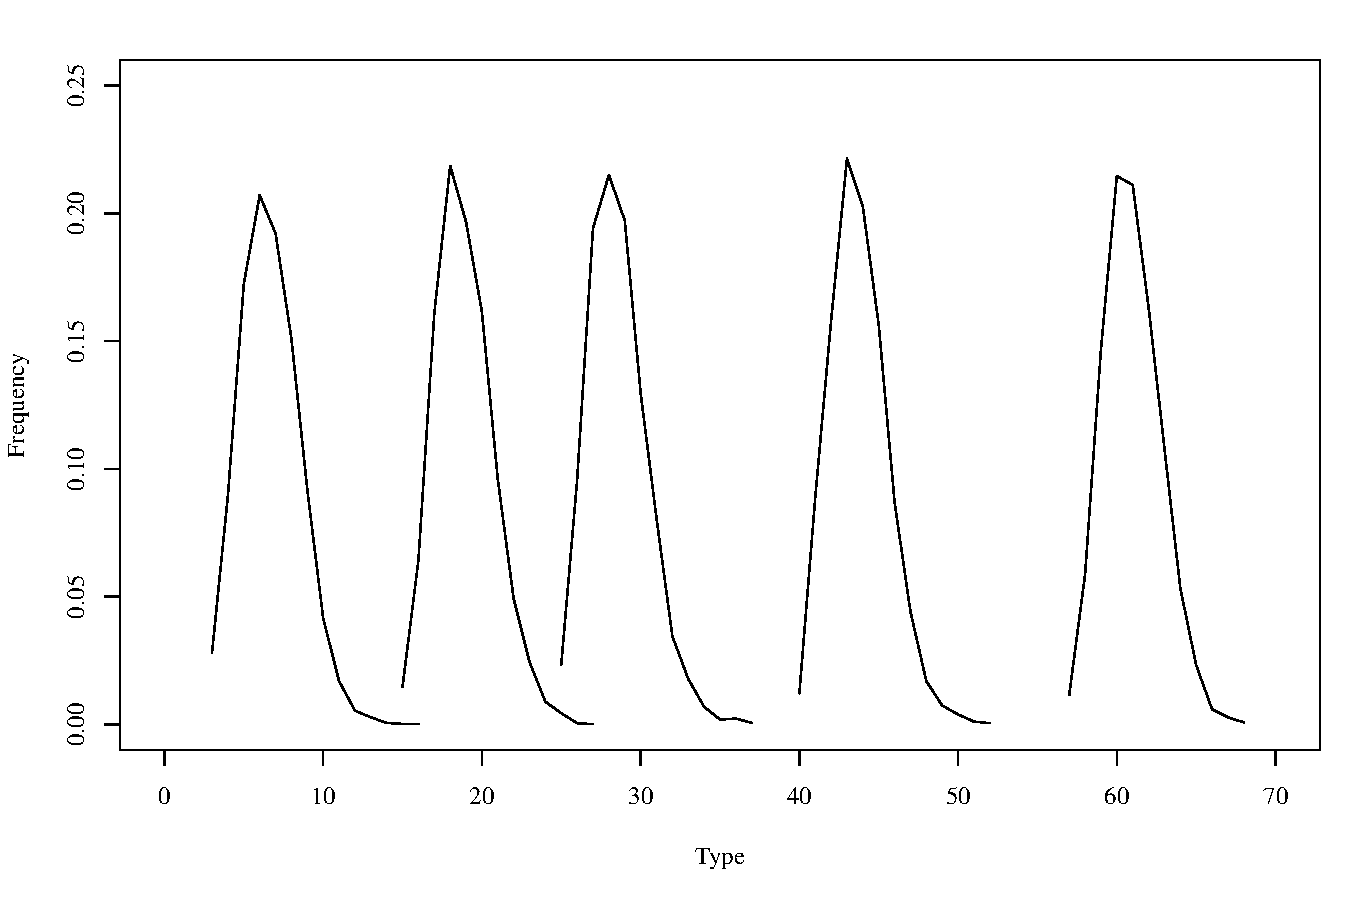
\includegraphics[width=14cm]{img/TravelingWave.pdf}
   \end{center}
  \caption{\label{mr:f:TravelingWave} The empirical distribution of types are
  drawn after $2N$, $10N$, $20N$, $30N$ and $40N$ generations respectively (from left to right).
   Here $N=10000$, $\lambda = 0.1$ and $\alpha =
  0.028$.}
\end{figure}
 
It is often useful to look at the vector of type frequencies $\RR$ relative to the current best
class, hence 
\[ \RRT{t} := \big(\mrKT{K^*(t)+k}{t}\big)_{k \in \N}, \]
as it forms a recurrent Markov chain on $\Simplex_N$. Therefore notice, that
mutation and selection are opposing each other in a way that the former always
increase the number of deleterious mutations while the latter tries to minimize
it. We will see that both forces drive the population towards a balance state.
We call such states equilibrium points. As we expect that $\mr$ stays in such a
point once it has reached it, we define them as follows.
\begin{Definition}
For a Markov chain $(\Vector{X}(t))_{t \in \N}$ on $\Simplex$, we call every
$\Vector{\pi} \in \Simplex$ with 
\[ \CE{\Vector{X}(t+1)}{\Vector{X}(t) = \Vector{\pi}} = \Vector{\pi} \]
an \emph{equilibrium point} (of $\Vector{X}$).
\end{Definition}

\noindent
However, the random fluctuations of genetic drift bars the population from
staying in an equilibrium point forever. In fact,
\citet{haigh_accumulation_1978} suggested that mutation and selection are strong
enough to dominate genetic drift when the ratchet is away from an equilibrium.
Therefore, the population drives towards an equilibrium point with strong force.
When it approaches this point, mutation and selection cancel each other out more
and more, and genetic drift becomes more important. Eventually, the random
fluctuations will lead to the extinction of the current best class, and the
ratchet clicks.

\noindent
Our main concern in this chapter is to prove that the Poisson distribution
with parameter $\theta$,
\begin{align} \label{mr:eq:pi}
\Vector{\pi} = \Vector{\pi}^0 := \left( e^{-\theta} \frac{\theta^k}{k!}
\right)_{k \in \N} \in \Simplex \qquad \text{with } \theta := \frac{\lambda}{\alpha},
\end{align}
and its right shifts $\Vector{\pi}^j$, so vectors with
\begin{align} \label{mr:eq:pi^j}
\pi^j_i = 
	\begin{cases}
	 0, & \text{if } i < j,\\
	 \pi_{i-j}, & \text{otherwise,} 
	\end{cases}
\end{align}
for $j \in \N$ are the equilibrium points of $\mr$. We state this as a theorem.
% 
\begin{Theorem} \label{mr:t:statp}
The equilibrium points of $\mr$ are exactly the distributions $\Vector{\pi}^j$
with $j \in \N$.
\end{Theorem}

\begin{proof}
``Uniqueness'' will be a consequence of Corollary~\ref{ips:c:conv} later. For
``existence'', let $j \in \N$. By Equation~\eqref{mr:eq:expectation} we have,
$$\CE{\mrKT{k}{t+1}}{\mrT{t} =
\Vector{\pi}^j} = 0 \qquad \text{for } k < j,$$ 

\noindent
and for $k \in \N$,
\begin{align*}
\CE{\mrKT{j+k}{t+1}}{\mrT{t} = \Vector{\pi}^j}
  &= \sum_{i=0}^{j+k} \frac{(1-\alpha)^{i} \cdot \pi^j_i }
  					   {\sum_{\ell=0}^\infty (1-\alpha)^\ell \pi^j_\ell} e^{-\lambda}
  					   \frac{\lambda^{(j+k-i)}}{(j+k-i)!} \\
 &= \sum_{i=0}^{k} \frac{(1-\alpha)^{i} \cdot \pi_i }
  					   {\sum_{\ell=0}^\infty (1-\alpha)^\ell \pi_\ell} e^{-\lambda}
  					   \frac{\lambda^{(k-i)}}{(k-i)!} \\ 			   
  &= \frac{e^{-\lambda}}{\sum_{\ell=0}^\infty \frac{(1-\alpha)^{\ell}
  \theta^\ell}{\ell!}}
     \sum_{i=0}^k \frac{(1-\alpha)^{i} \theta^i}{i!}
     \frac{\lambda^{(k-i)}}{(k-i)!}  \\
  &= \frac{e^{-\lambda}}{e^{(1-\alpha)\theta}}
  	 \frac{\lambda^k}{k!} 
  	 \sum_{i=0}^k \left( \frac{(1-\alpha) \theta}{\lambda} \right)^i
  	 \frac{k \cdot \ldots \cdot (k-i+1)}{i!} \\
  &= e^{-(\lambda \alpha^{-1} (1-\alpha) + \lambda)}
     \frac{\lambda^k}{k!}
     \left( \frac{(1-\alpha)}{\alpha} + 1 \right)^k \\
  &= e^{-\theta} \frac{\theta^k}{k!}. \qedhere
\end{align*}
\end{proof}

\noindent
To prove the ``uniqueness'' of the $\Vector{\pi}^j$, we examine the convergence
behavior of an approximation of Muller's ratchet, the ratchet without the effects of genetic drift. By the above argumentation, this
approximation never clicks, and therefore will give us an impression of the ratchet's behavior in
the time between two clicks.

\section{The Approximation With Infinite Population Size}
One of the first ideas in the examination of Muller's ratchet was to simplify the model by ignoring
the effects of genetic drift. Therefore notice that according to the law of large numbers,
$\mrKT{k}{t+1}$ becomes almost surely deterministic if we increase the population size $N$ towards
infinity. We take this as motivation for the following definition.

\begin{Definition} \label{dips:def:mrips}
Let $\lambda > 0$, $\alpha \in [0,1)$ and $\Vector{x} \in \Simplex$.  
We call the time discrete, deterministic process $\mrIpsT{t} = (\mrIpsKT{i}{t})_{i \in
\N}$ with $\mrIpsT{0} = \Vector{x}$ and 
\begin{align*}
\mrIpsKT{k}{t+1} := p_k(t) = 
	\sum_{i=0}^k \frac{(1-\alpha)^{i} \cdot \mrIpsKT{i}{t}}{W(t)}
				 e^{-\lambda} \frac{\lambda^{(k-i)}}{(k-i)!}
\end{align*}
the \emph{large population limit} of Muller's ratchet.
\end{Definition}

\noindent
As $\mrIps$ and $\mr$ equal each other in (conditioned) expectation, they have exactly the same
equilibrium points. Hence, we already know from Theorem~\ref{mr:t:statp} that all right shifts of
$\Vector{\pi}$ are equilibrium points of $\mrIps$ as well. In return, we use the more simple
deterministic process to prove the absence of other equilibrium points. As the
almost sure convergence implies convergence in distribution, we can furthermore
assume that the claimed approximating behavior holds.

The large population limit of Muller's ratchet is in particular useful because the recursion given
by Definition~\ref{dips:def:mrips} has been explicitly solved by \citet{maia_analytical_2003}.

\begin{Theorem}[\cite*{maia_analytical_2003}] \label{ips:t:maia}
For all $t \in \N$,  $\mrIpsT{t}$ is given by
\begin{equation} \label{ips_explicit}
\mrIpsKT{k}{t} = \frac{\exp(-\theta_t)}{\sum_{j=0}^\infty
\mrIpsKT{j}{0} \, (1-\alpha)^{j t}}
\sum_{j=0}^k \frac{\theta^{k-j}_t}{(k-j)!} \mrIpsKT{j}{0} (1-\alpha)^{j t},
\end{equation}
where $\theta_t = \frac{\lambda}{\alpha}\left[ 1 - \left(1-\alpha\right)^t \right] $.
\end{Theorem}
\begin{proof}
The proof is based on the fact that we can uniquely determine a discrete probability distribution
$\Vector{x} \in \Simplex$ by its \emph{generating function}
\[ G[z,\Vector{x}] := \sum_{i=0}^\infty x_i z^i, \qquad z \in [0,1] \]
(e.g. see \citet[Chapter 3]{klenke_wahrscheinlichkeitstheorie_2006}). Hence, we translate
$\mrIpsT{t}$ into terms of generating functions, solve the recursion there and translate the
solution back to a probability distribution afterwards.

\noindent
First, notice that
\[ G[1-\alpha, \mrIpsT{t}] = \sum_{i=0}^\infty \mrIpsKT{i}{t} (1-\alpha)^i = W(t). \]
Using the equation
\begin{align} \label{ips_Maia_NR}
\sum_{i=j}^\infty e^{-\lambda} \frac{\lambda^{i-j}}{(i-j)!} z^i
=  e^{-\lambda} z^j \sum_{i=0}^\infty \frac{(\lambda z)^i}{i!}
=  z^j e^{\lambda(z-1)}
\end{align}
we obtain the recursion
\begin{equation}
\begin{aligned}
G[z,\mrIpsT{t+1}]
& =  \sum_{i=0}^\infty \mrIpsKT{i}{t+1} z^i \\
& =  \sum_{i=0}^\infty \sum_{j=0}^i \frac{(1-\alpha)^j \mrIpsKT{j}{t}}{W(t)}
e^{-\lambda} \frac{\lambda^{i-j}}{(i-j)!} z^i \\
& =  \sum_{j=0}^\infty \sum_{i=j}^\infty \frac{(1-\alpha)^j \mrIpsKT{j}{t}}{W(t)}
e^{-\lambda} \frac{\lambda^{i-j}}{(i-j)!} z^i \\
& =  \sum_{j=0}^\infty \frac{(1-\alpha)^j \mrIpsKT{j}{t}}{W(t)} \sum_{i=j}^\infty
\frac{\lambda^{i-j}}{(i-j)!} z^i \\
& =  \sum_{j=0}^\infty \frac{(1-\alpha)^j \mrIpsKT{j}{t}}{W(t)} z^j e^{\lambda(z-1)} \\
& =  e^{\lambda(z-1)} \frac{G[z(1-\alpha),\mrIpsT{t}]}{G[(1-\alpha),\mrIpsT{t}]}
\label{ips_RecursiveGenFunction}
\end{aligned}
\end{equation}
where we can reorder the summands because they are all non-negative.
We use \eqref{ips_RecursiveGenFunction} to prove by induction that
\begin{equation} \label{ips_ExplicitGenFunction}
G[z,\mrIpsT{t}] = e^{\theta_t (z-1)} \,
\frac{G[z(1-s)^t,\mrIpsT{0}]}{G[(1-\alpha)^t,\mrIpsT{0}]} .
\end{equation}
While (\ref{ips_ExplicitGenFunction}) is obvious for
$t=0$, we have
\begin{align*}
G[z,\mrIpsT{t+1}]
&\stackrel{\eqref{ips_RecursiveGenFunction}}{=} e^{\lambda (z-1)} \,
\frac{G[z(1-\alpha),\mrIpsT{t}]}{G[1-\alpha,\mrIpsT{t}]} \\
&\stackrel{\eqref{ips_ExplicitGenFunction}}{=} e^{\lambda (z-1)} \,
\frac{e^{\theta_t (z(1-\alpha)-1)} \cdot G[z(1-\alpha)^{t+1},\mrIpsT{0}]}
{e^{\theta_t ((1-\alpha)-1)} \cdot G[(1-\alpha)^{t+1},\mrIpsT{0}]} \\
& =  e^{ \lambda (z-1) + \theta_t (z (1-\alpha) -1) + \theta_t \alpha } \,
\frac{G[z(1-\alpha)^{t+1},\mrIpsT{0}]}{G[(1-\alpha)^{t+1},\mrIpsT{0}]} \\ 
& = e^{\theta_{t+1}(z-1)} \,
\frac{G[z(1-\alpha)^{t+1},\mrIpsT{0}]}{G[(1-\alpha)^{t+1},\mrIpsT{0}]}
\end{align*}
because
\begin{align*}
\lambda (z-1) + \theta_t(z (1-\alpha) -1) + \theta_t \alpha
& = \frac{\lambda}{\alpha} \left( z-z(1-\alpha)^{t+1}-1+(1-\alpha)^t-\alpha(1-\alpha)^t \right) \\
& = \frac{\lambda}{\alpha} \left( z-z(1-\alpha)^{t+1}-1+(1-\alpha)^{t+1} \right) \\
& = (z-1) \, \frac{\lambda}{\alpha} (1-(1-\alpha)^{t+1}).
\end{align*}

\noindent
Finally, we again write \eqref{ips_ExplicitGenFunction} as a generating
function to identify its coefficients.

{\allowdisplaybreaks
\begin{align*}
G[z,\mrIpsT{t}] & = e^{\theta_t (z-1)} \,
\frac{G[z(1-\alpha)^t,\mrIpsT{0}]}{G[(1-\alpha)^t,\mrIpsT{0}]} \\ 
& = \frac{1}{G[(1-\alpha)^t,\mrIpsT{0}]} \sum_{j=0}^\infty \mrIpsKT{j}{0} (1-\alpha)^{j t} z^j
e^{\theta_t (z-1)} \\
& \stackrel{\eqref{ips_Maia_NR}}{=}
\frac{1}{G[(1-\alpha)^t,\mrIpsT{0}]} \sum_{j=0}^\infty \mrIpsKT{j}{0} (1-\alpha)^{j t}
\sum_{k=j}^\infty \frac{\theta_t^{k-j}}{(k-j)!} z^k e^{-\theta_t} \\
& = \frac{1}{G[(1-\alpha)^t,\mrIpsT{0}]} \sum_{j=0}^\infty \sum_{k=j}^\infty \mrIpsKT{j}{0}
(1-\alpha)^{j t} \frac{\theta_t^{k-j}}{(k-j)!} z^k e^{-\theta_t} \\
& = \frac{1}{G[(1-\alpha)^t,\mrIpsT{0}]} \sum_{k=0}^\infty \sum_{j=0}^k \mrIpsKT{j}{0}
(1-\alpha)^{j t} \frac{\theta_t^{k-j}}{(k-j)!} z^k e^{-\theta_t} \\
& = \sum_{k=0}^\infty \left( \frac{e^{-\theta_t}}{G[(1-\alpha)^t,\mrIpsT{0}]}  \sum_{j=0}^k
\mrIpsKT{j}{0} (1-\alpha)^{j t} \frac{\theta_t^{k-j}}{(k-j)!} \right) z^k \\
& = \sum_{k=0}^\infty \left( \frac{e^{-\theta_t}}{\sum_{j=0}^\infty
\mrIpsKT{j}{0} (1-\alpha)^{j t}}  \sum_{j=0}^k
\mrIpsKT{j}{0} (1-\alpha)^{j t} \frac{\theta_t^{k-j}}{(k-j)!} \right) z^k \qedhere
\end{align*} }
\end{proof}

\noindent
Note that by \eqref{ips_explicit}, $\mrIpsKT{k}{t} = 0$ if and only if $\mrIpsKT{j}{0} = 0$ for all
$j \leq k$. Hence -- as argued above -- the large population limit of Muller's ratchet never clicks.

Using Theorem~\ref{ips:t:maia}, we can both prove the uniqueness in Theorem~\ref{mr:t:statp} and show that
the equilibrium points attract Muller's ratchet with infinite population size.  We define
$\Vector{y}$ for $\mrIps$ as $\RR$ for $\mr$, i.e. as the type frequencies relative to the fittest
class.

\begin{Corollary} \label{ips:c:conv}
For any starting distribution $y(0)$ and $k \in \N$, we have $y_k(t) \Conv
\pi_k$ for $t \Conv \infty$. In particular, $\Vector{\pi}$ is the only
equilibrium point for $\Vector{y}$.
\end{Corollary}
\begin{proof}
Recall from Theorem~\eqref{ips:t:maia} that
\begin{equation} \label{dips:eq:expl2}
y_k(t) = \frac{\exp(-\theta_t)}{\sum_{j=0}^\infty
y_j(0) \, (1-\alpha)^{j t}}
\sum_{j=0}^k \frac{\theta^{k-j}_t}{(k-j)!} y_{j}(0) (1-\alpha)^{j t}.
\end{equation}
Obviously $\theta_t = \theta \left[ 1 - \left(1-\alpha \right)^t \right] \Conv
\theta$. As the following calculation shows, the sums in (\ref{dips:eq:expl2}) are dominated by their
$y_{0}(0)$ term:
\[
0 \leq
\lim_{t \to \infty} \sum_{j=1}^\infty y_{j}(0)(1-\alpha)^{j t} \leq
\lim_{t \to \infty} \sum_{j=1}^\infty \left( \left(1-\alpha \right)^{t} \right)^j =
\lim_{t \to \infty} \frac{1}{1-(1-\alpha)^t} - 1 = 0
\]
and
\[
0 
\leq \lim_{t \to \infty} \sum_{j=1}^k \frac{\theta^{k-j}_t}{(k-j)!} y_{j}(0)
	(1-\alpha)^{j t}
\leq e^\theta \lim_{t \to \infty} \sum_{j=1}^\infty \left( \left(1-\alpha
	\right)^{t} \right)^j =
0
\]
using the limit of the geometric series for $\left(1-\alpha \right)^{t}$ and
the fact that $\frac{\theta_t^{k-j}}{(k-j)!} \leq e^{\theta_t} \leq e^\theta $.

\noindent
Hence we have
\begin{align*}
\lim_{t \to \infty} y_{k}(t) &=
\lim_{t \to \infty} \frac{\exp(-\theta_t)}{\sum_{j=0}^\infty y_{j}(0) \,
(1-\alpha)^{j t}} \sum_{j=0}^k \frac{\theta^{k-j}_t}{(k-j)!} y_{j}(0)
(1-\alpha)^{j t} \\
&= \frac{\exp(-\theta)}{y_{0}(0)}
\frac{	\theta^k}{k!} y_{0}(0) \\
&= \frac{\theta^k}{k!} \exp(-\theta) 
\end{align*}
where the second equality is valid because $y_0(0) > 0$ by definition.
\end{proof}

\noindent
Taking \eqref{mr:eq:recurrence} into account, we conclude that the ratchet with infinite
population size with best class $k$ will always tend towards
$\Vector{\pi}^{k}$. If the population size $N$ is big enough, the ratchet with
finite population size should behave similarly. However, after a click --
which should occur only rarely for such $N$ -- the ratchet will tend to
$\Vector{\pi}^{k+1}$ instead. 

The question which values of $N$ are actually ``big enough'' for different
combinations of $\lambda$ and $\alpha$ is unanswered yet. However, as the large
population limit does not click, $N$ surely is too small if Muller's ratchet
clicks frequently. Different authors made predictions for when this should be
the case. For example, \cite{haigh_accumulation_1978} suggested that the ratchet
clicks frequently if the expected size of the best class $n_0 = N e^{-\theta}$
is less than one individual, while \cite{etheridge_how_2008} concluded that the
same should occur if $\frac{N \lambda}{N \alpha \cdot \log(N\lambda)}$ is less then $0.5$.
Anyway, the magnitude of the ``finite population effect'' seems to be closely
related to the click rate of the ratchet.